% !TeX root = ../main.tex

\chapter{编译器前端}
\section{抽象语法树}
\subsection{AST简介}
通常而言,编译器前端的主要流程是:先读取源代码文件中的字符流,然后通过词法分析生成token流,再通过语法分析生成抽象语法树(AST),最后将AST转换为与编程语言无关的IR送往中段,进行各种通用优化。

AST是程序结构的一种抽象表示,以树的形式表现编程语言的语法结构,树上的每个节点都表示源代码中的一种结构,如本项目中的类sysyParaser定义了以下结构性AST节点:

\begin{table}[htb]
  \centering\small
  \caption{源码结构的抽象语法树}
  \label{tab:ast1}
  \begin{tabular}{cl}
    \toprule
    AST node   & 描述                                       \\
    \midrule
    CompUnit & 编译单元,即源文件\\
    FuncDef & 函数声明,对应唯一函数名 \\
    Block & 大括号作用域 \\
    SelectStmt & if语句的语法结构 \\
    LoopStmt & while语句的语法结构 \\
    \bottomrule
  \end{tabular}
\end{table}
这些结构都会直接翻译到HIR。对于指令和操作数对应的节点,这里以声明和赋值语句为例:

\begin{table}[htb]
  \centering\small
  \caption{声明和赋值语句的抽象语法树}
  \label{tab:ast2}
  \begin{tabular}{cl}
    \toprule
    AST node   & 描述                                       \\
    \midrule
    VarDecl & 声明语句,如int\space a\\
    VarDef:int & 声明的作用域内唯一的变量名\\
    AssignStmt & 赋值语句,如a\space =\space 1\\
    Lval & 左值,查找作用域最近的左值变量的名称\\
    AddExp & 加法的优先级最低   \\
    MulExp & 乘法优先级较高 \\
    ArrayExp & 数组取元素优先级高于算数运算 \\
    FuncExp & 函数作用符优先级最高 \\
    Number & 立即数\\

    \bottomrule
  \end{tabular}
\end{table}


\subsection{AST节点生成举例}

指令$\text{var} = 10+4*f(\text{a[0]})$ 经过词法分析和语法分析后得到的AST表示如图:

\begin{figure}[htb]
  \centering
  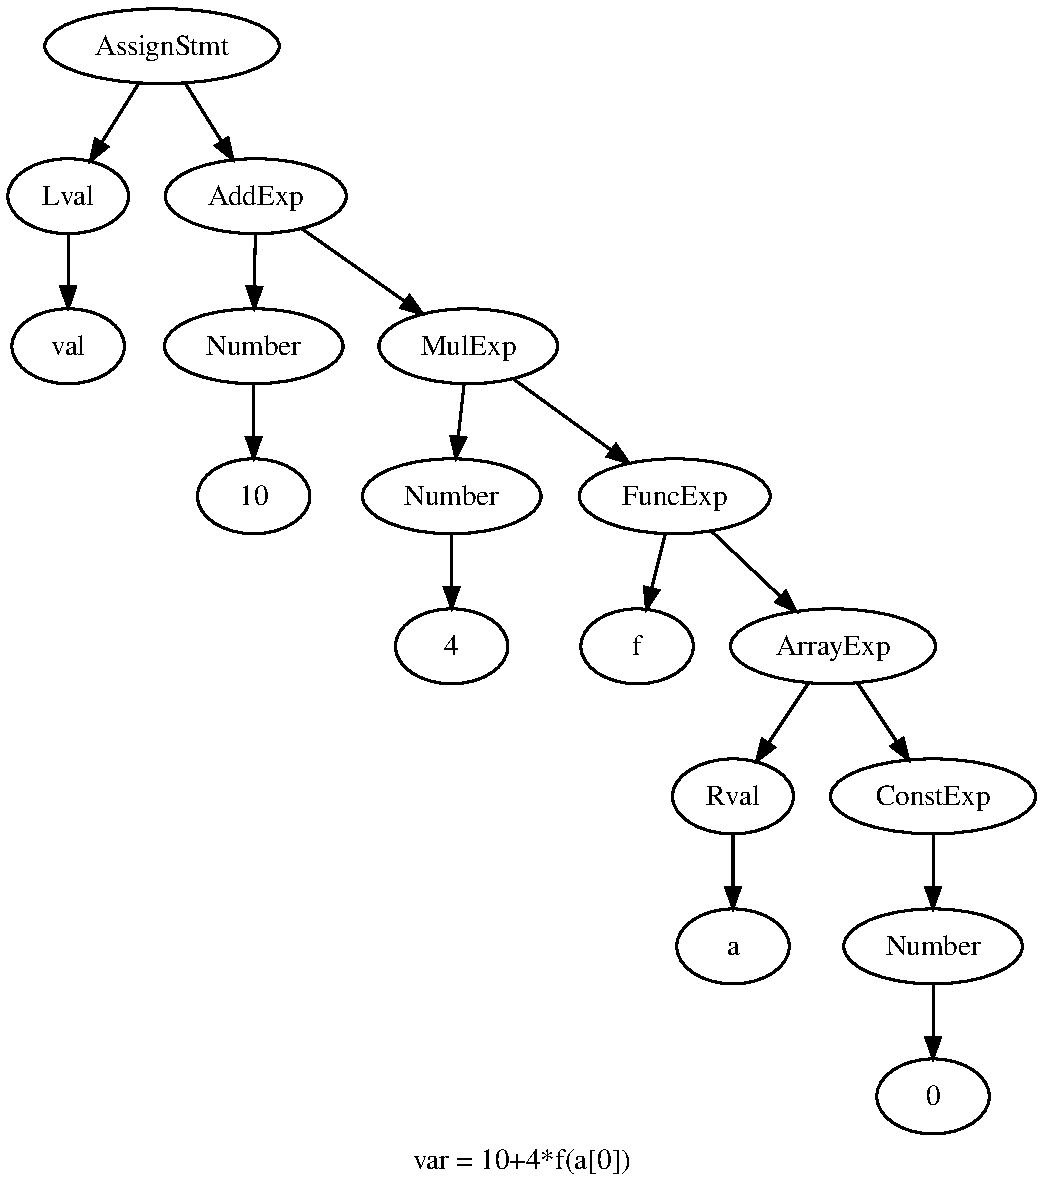
\includegraphics[width=0.9\textwidth]{figures/ASTnode.pdf}
  \label{fig:astnode}
\end{figure}



抽象语法树保留了源程序的结构性信息,适合转换为IR。

\section{生成中间表示}
\subsection{中间表示简介}
抽象语法树可以转换为更容易进行分析变换的中间形式 IR,好的IR设计应该满足如下特点:

1. 容易从AST转换得来

2. 利于进行各种通用优化

3. 容易转换到各种平台的机器码

为了对应以上三个需求,本项目提出了三层IR的设计,即利于从AST得到,保留结构性信息的高层IR,利于优化的中层IR,和直接对应到比赛测试平台目标机器底层架构的底层IR,如图~\ref{fig:threeIR}。

\begin{figure}[htb]
  \centering
  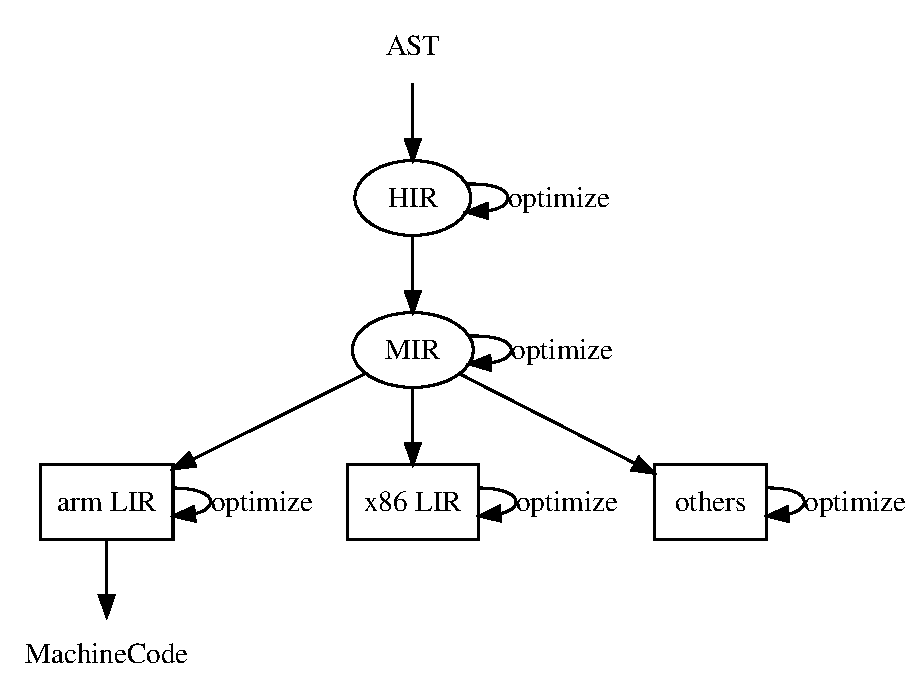
\includegraphics[width=1.0\textwidth]{figures/three_layer_IR.dot.pdf}
  \caption{三层IR的示意图}
  \note{高层IR保留结构信息,利于从AST变换,中层IR即通常意义上与机器和语言无关的中间表示,利于优化,底层IR与特定架构相结合,进一步提高优化效果,生成目标机器码。}
  \label{fig:threeIR}
\end{figure}

\subsubsection{高层IR}

设计上保留了源代码 if while 等结构的信息,方便结构级变换。在该层的主要分析和优化有:


AccumulatePattern:累加变量外提

HighIRsimplyCFG:高层IR上的流程图简化

LoopMerge:while 循环合并

MergeCond:嵌套 if 条件块合并

\subsubsection{中层IR}
中层IR设计上接近 LLVM IR,适合于各类通用优化,是本文论述的重点,在该层的主要分析和优化有:

ActiveVars   活跃变量分析

BBCommonSubExper   块内公共子表达式消除

BBConstPropagation   块内常量传播

BranchMerge  分支合并

CondSimplify  条件块简化合并

ConstFlod  常量折叠

ConstLoopExpansion  循环展开

DeadCodeEliminate  死代码删除

Dominators  支配树分析

FunctionInline  简易函数内联

IRCheck  检测 IR 的数据结构是否有不一致

LoopFind  循环查找

LoopInvariant  循环不变量外提

Multithreading   循环多线程化

PowerArray  将特殊形式数组的访问替换为计算

ReachDefinition  到达定值分析

RefactorParlins  交换操作数位置

SimplifyCFG  基本块合并与删除

Mem2Reg  半剪枝算法构造 SSA 形式 IR


\subsubsection{低层IR}

如上方图~\ref{fig:threeIR},LIR设计上贴近硬件架构,舍弃了移植性但是进一步利用ARM架构的特征提高了性能,与后端相配合共同完成指令融合、调度和选择等优化。

InstructionSchedule: 指令调度软流水

LowerIR:将中层 IR 翻译到低层 IR 并在上面做一系列相关优化,如针对数组寻址利用ARM架构的加法和位移“融合”指令来减少指令数,针对高中层的求余指令翻译到ARM架构的实际运算指令,消除不被用到的操作数等等。

RegisterAllocation: 寄存器分配

\subsection{访问者模式生成IR}

访问者模式是一种行为设计模式,能够将算法操作(访问者)与其被作用的将对象(被访问者)分离,适用于对象本身具有复杂结构且对象相对固定但需要频繁增加对于对象的操作的场景。在编译器设计中访问者对应于对象IRBuilder,被访问者即由词法和语法解析器生成的AST,IRBuilder通过visit方法访问AST,AST对象通过accept方法接受访问。 

在编译器前端完成词法分析将SysY源代码程序转换token流,再完成语法分析将token流构建为AST之后,需要对AST做多次遍历,如建立函数和全局变量列表、合法性检查、转换至IR。

下面介绍对IRBuilder的伪代码。

\begin{algorithm}[htb]
  \small
  \SetAlgoLined
  \KwData{syntax tree visitor of a Module}
  \KwResult{Build Hight IR}
  initialization\;
  Create TyInt32\;
  Create TyInt1/Bool\;
  Create TyInt32Ptr\;
  Create Void\;
  \While{List<DeclDef> not empty}{
    visit DeclDef\;
  }
  \caption{访问模块生成IR}
  \label{algo:algorithm1}
\end{algorithm}

当模块中的DeclDef子语法树节点在接受访问时,除了不创建Void,32位整数,32位整数指针,布尔变量这四个全局唯一的类型外,其他代码相同,即对其语法树的子节点,深度优先遍历,直到叶节点。以函数语法节点的遍历为例:在函数的IR建立过程中,编译器分析参数类型和参数列表,函数返回值,变量名称何其作用域,根据AST的语法结构创建HIR指令序列。

\subsection{HIR生成示例}

如以下代码文件:

\begin{verbatim}
    int main() {
      int b = 10;
      int c;
      if (b>0){
    	  c = b+4;  
      }
      else {
    	  c = 0;
      }
      return c;
    }
\end{verbatim}

整个文件经过词法分析和语法分析后,得到抽象语法树表示如图~\ref{fig:AST}:

\begin{figure}[htb]
  \centering
  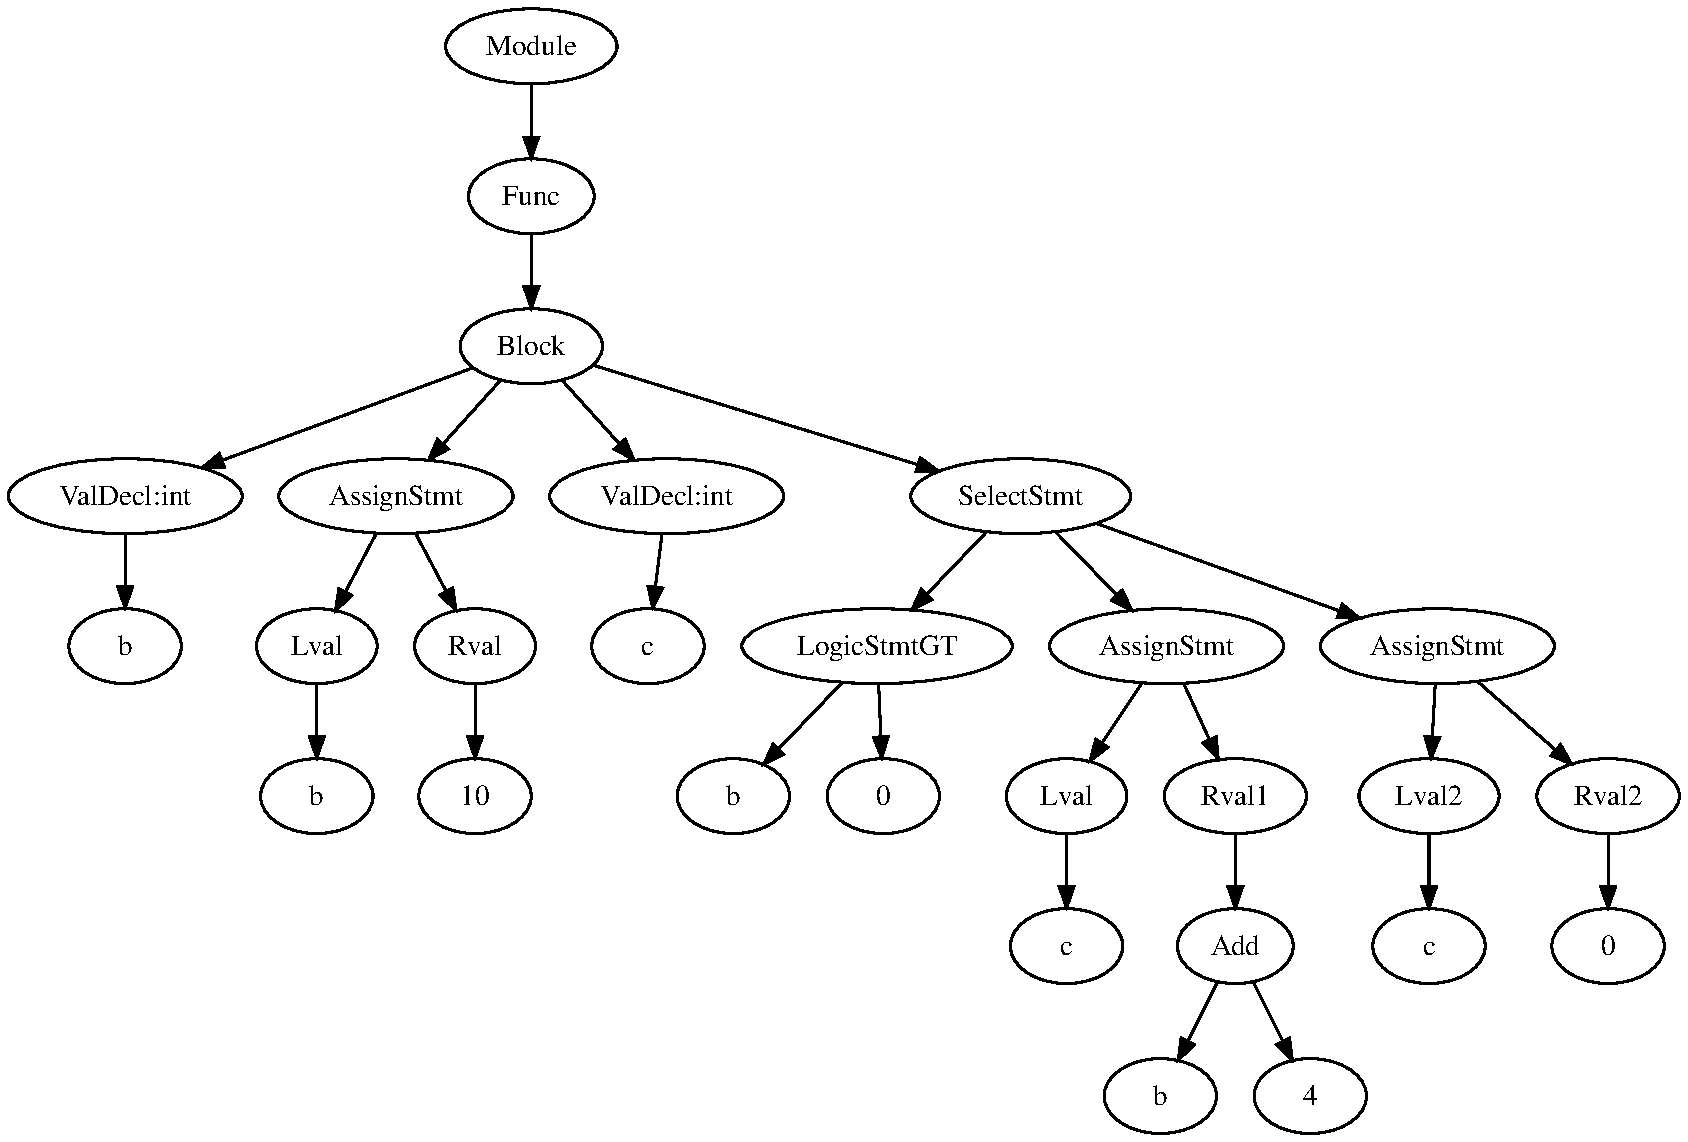
\includegraphics[width=0.9\textwidth]{figures/ast.pdf}
  \caption{抽象语法树的形式}
  \label{fig:AST}
\end{figure}

AST的根节点Module即整个编译文件,由于该文件内仅定义了一个函数main,所以根节点只有一个子节点Func,在High IR层级,因为需要保留程序的结构性信息,也为了降低从AST得到HIR的难度,所以HIR定义的并不是基本块,项目定义了保留结构性信息的Base Block,If Block或While Block,在经过HIR到MIR的转换时再生成Basic Block。因而经过IRBuilder之后生成的HIR图~\ref{fig:HIR}中仅有顺序执行的Block。

HIR会保留if或者while等控制流结构,虽然方便从语法树中的SelectStmt部分直接得来,但是无法体现出控制流的动态流动。事实上,第二个Block会在转换到MIR时对三个部分进行拆分。

\begin{figure}[htb]
  \centering
  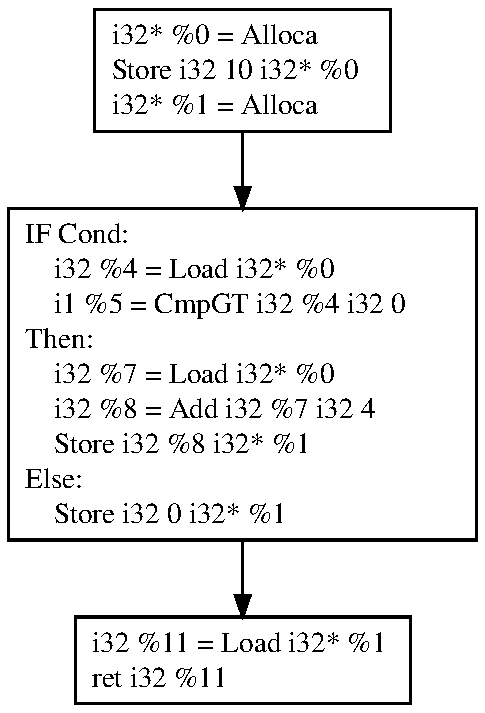
\includegraphics[width=0.5\textwidth]{figures/HIR.pdf}
  \caption{HIR示例}
\label{fig:HIR}
\end{figure}

其中源代码变量的define和use与虚拟寄存器的对应如表~\ref{tab:compare}

\begin{table}[htb]
  \centering\small
  \caption{虚拟寄存器和源代码变量对照表}
  \label{tab:compare}
  \begin{tabular}{cl}
    \toprule
    virtual register  & define or use   \\
    \midrule
    \%0 & 变量b的声明 \\
    \%1 & 变量c的声明 \\
    \%4 & if的条件使用了变量b \\
    \%5 & if的结果布尔值的声明 \\
    \%7 & add的操作数使用了变量b \\
    \%8 & add的结果的声明 \\
    \%11 & 返回语句的参数使用了变量c \\
\bottomrule
  \end{tabular}
\end{table}

\subsection{中间表示组织}
理解中间形式的组织和表示方式是理解整个项目甚至是以LLVM为代表的现代编译器设计理论的基础和关键,IR 按照如下层级关系进行组织:

1. Module : 编译的单元,通常是整个文件 

2.Function : 源码中的某个函数,通常是为完成某种功能的封装   

3.Basic Block : 函数中一个只能在结尾处跳转,在入口处进入的指令集合       

4.Instruction : 基本块中的某条最基本的指令,是IR执行的最小单位


同时,为了方便后续编译器的优化,编译器会花费大量的篇幅用于索引和遍历函数,基本块,甚至是指令的操作数,因此为这些数据结构设置C++风格的“迭代器”(Iterators)是有必要的,也是符合 IR 的组织形式的,它们的迭代器及其作用如下:

1. Module::iterator 对编译的单元,迭代其内部的所有函数

2. Function::iterator 对某个函数,遍历构成其的基本块集合

3. BasicBlock::iterator 对某个基本块,顺序遍历其内部的指令

这四种迭代器的设计是对IR的层级架构的直观表达。本项目的输入文件是一个sy文件,对应一个Module,一个文件内可以定义几个函数,这对应若干个该Module内的Function,一个函数内乍看起来是一定数目的指令,但是直接对控制流复杂的函数进行分析并不方便。基本块是只能从其第一条指令进入,从最后一条指令结束执行,中间不能发生跳转的指令集和,基本块在循环识别,数据流分析等优化中都有重要作用,因此我们采用包含若干条指令的基本块作为函数迭代的结果。而对基本块的遍历就是其中的顺序流指令。